\documentclass[a4paper,article,14pt]{extarticle}

\usepackage{spbudiploma}
\usepackage{amsmath}
\usepackage{mathtools}
\usepackage[pdftex]{graphicx}
\graphicspath{{../pictures/}}
\usepackage{listings}
\usepackage{xcolor}
\usepackage{amsfonts}
\usepackage{amsmath}
\usepackage{cases}

\usepackage{enumitem}
\definecolor{codegreen}{rgb}{0,0.6,0}
\definecolor{codegray}{rgb}{0.5,0.5,0.5}
\definecolor{codepurple}{rgb}{0.58,0,0.82}
\definecolor{backcolour}{rgb}{0.95,0.95,0.92}

\lstdefinestyle{mystyle}{
	backgroundcolor=\color{backcolour},   
	commentstyle=\color{codegreen},
	keywordstyle=\color{codegreen},
	numberstyle=\tiny\color{codegray},
	stringstyle=\color{codepurple},
	basicstyle=\ttfamily\footnotesize,
	breakatwhitespace=false,         
	breaklines=true,                 
	captionpos=b,                    
	keepspaces=false,                 
	numbers=left,                    
	numbersep=5pt,                  
	showspaces=false,                
	showstringspaces=false,
	showtabs=false,                  
	tabsize=2
}

\lstset{style=mystyle}

\begin{document}
	\begin{titlepage}
		\begin{center}
			FEDERAL STATE AUTONOMOUS EDUCATIONAL INSTITUTION
			
			OF HIGHER EDUCATION
			
			ITMO UNIVERSITY
			\vspace{3cm}
			
			\large\textbf{Report}
			
			\large on the practical task No. 7
			
			\large \flqq Algorithms on graphs. \\ Tools for network analysis\frqq
			\vspace{5cm}
			

			\begin{flushright}
				{Performed by:} \\
				Putnikov Semyon \\ 
				J4132c \\
			\end{flushright}
			
			
			\begin{flushright}
				{Accepted by:} \\
				Dr Petr Chunaev \\ 
			\end{flushright}
			\vfill
			
			{St. Petersburg}
			\par{\number\year}
		\end{center}
	\end{titlepage}

	\newpage
	
	\section{Goal}
	The use of the network analysis software Gephi.
	
	\section{Problems and methods}
	\begin{enumerate}
		\item Download and install Gephi from https://gephi.org/.
		\item Choose a network dataset from https://snap.stanford.edu/data/ with number of nodes at most 10,000. You are free to choose the network nature and type (un/weighted, un/directed).
		\item Change the format of the dataset for that accepted by Gephi (.csv, .xls, .edges, etc.), if necessary.
		\item Upload and process the dataset in Gephi. Check if the parameters of import and data are correct.
		\item Obtain a graph layout of two different types.
		\item Calculate available network measures in Statistics provided by Gephi.
		\item Analyze the results for the network chosen.
	\end{enumerate}

	While performing the work, screenshot the main steps you are doing and insert in the report.
	
	\section{Results}
	%Present the results of solving the assigned problems, including graphs and tables, as well as a brief discussion of the results obtained (at most 4 pages)
	
	Arxiv GR-QC (General Relativity and Quantum Cosmology) collaboration network is from the e-print arXiv and covers scientific collaborations between authors papers submitted to General Relativity and Quantum Cosmology category.
	
	\subsection{Make graph from data}
	
	Initial data was txt file with structure: “node \t node” on each row that means a edge of the graph. Preprocessing:
	\begin{enumerate}
		\item Rename header to Source, Target.
		\item Replace all tabs with comma to make csv file.
	\end{enumerate}

	Now we can open our data as graph in Gephi.

	\begin{figure}[h!]
		\centering
		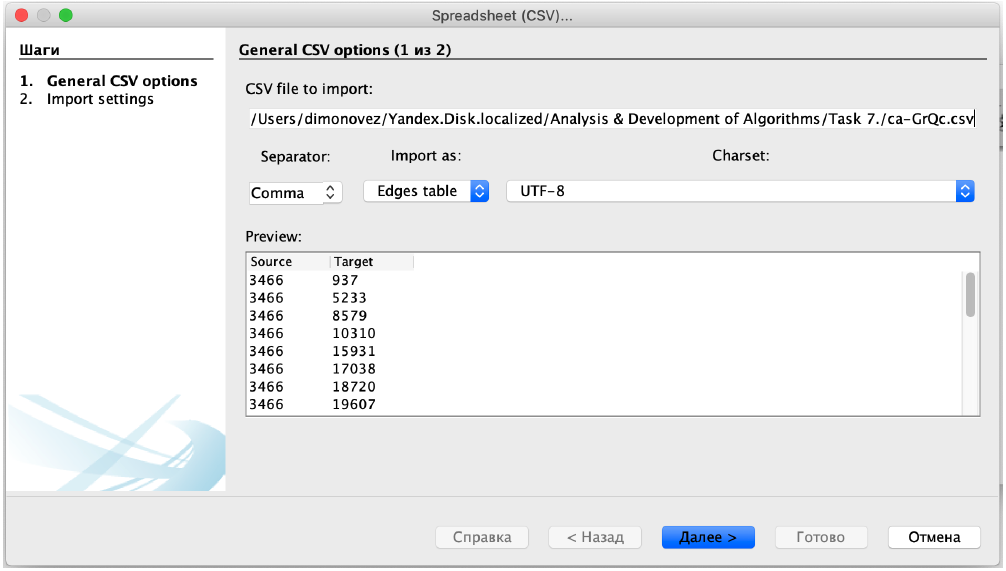
\includegraphics[scale=0.5]{import.png}
		\caption{Import data.}
		\label{graph}
	\end{figure}

	\begin{figure}[h!]
		\centering
		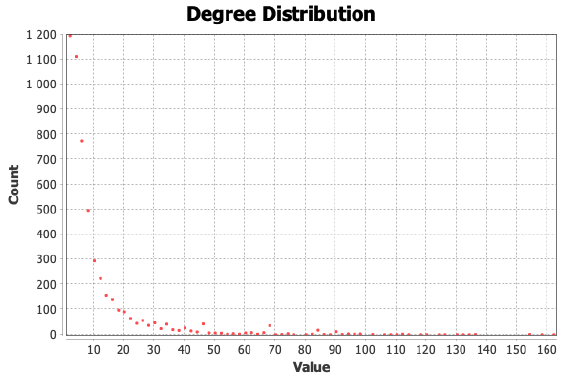
\includegraphics[scale=0.5]{degree.png}
		\caption{Degree Distribution.}
		\label{degree}
	\end{figure} 

	\begin{figure}[h!]
		\centering
		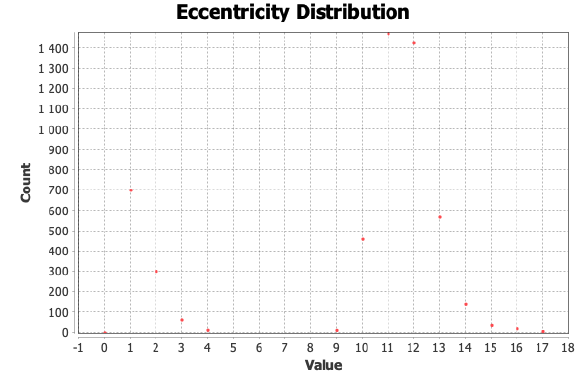
\includegraphics[scale=0.5]{eccentricity.png}
		\caption{Eccentricity Distribution.}
		\label{eccentricity}
	\end{figure} 

	\begin{figure}[h!]
		\centering
		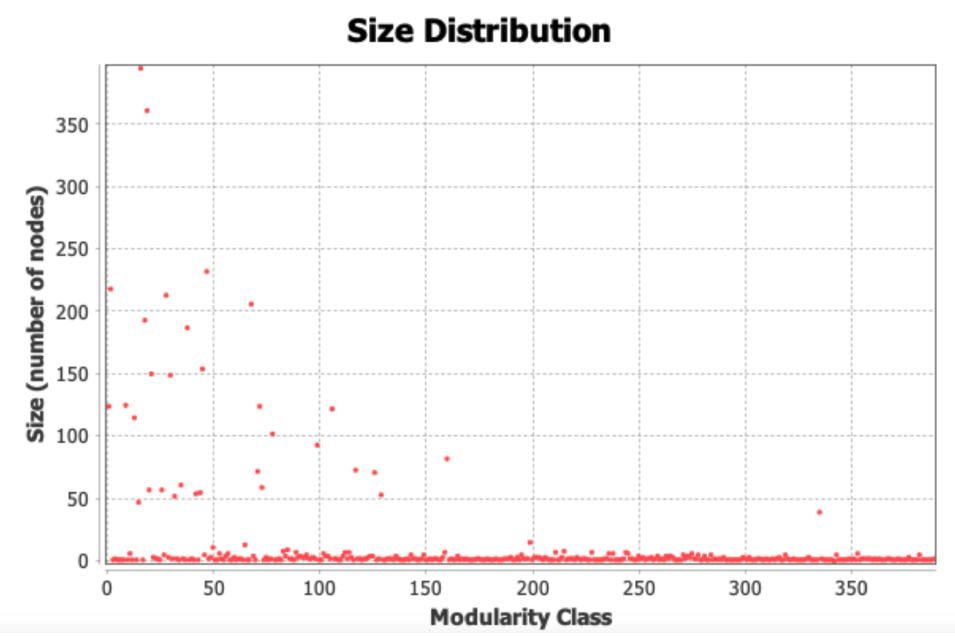
\includegraphics[scale=0.35]{size.png}
		\caption{Size Distribution.}
		\label{size}
	\end{figure} 

	\begin{figure}[h!]
		\centering
		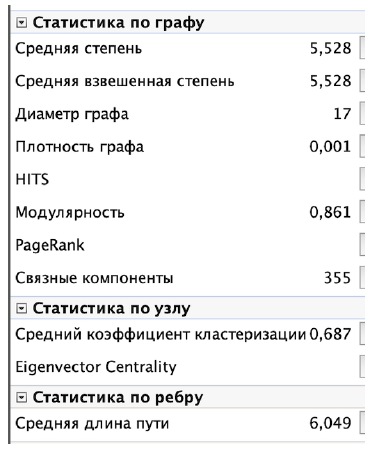
\includegraphics[scale=0.35]{statistic.png}
		\caption{Statistics.}
		\label{stat}
	\end{figure} 

	In each of the graph layouts we can see that graph have many connectivity components. That means that authors in each component are closely related and are not published with anyone else.
	
	\subsection{Statistics}
	
	\begin{itemize}
		\item $|V|=5242$
		\item $|E|=14496$
		\item Average degree: 5.528
		\item Diameter: 17
		\item Average path length: 6.05
		\item Radius: 1
		\item Density of the graph: 0.001 (Sparse)
		\item Modularity: 0.861
		\item Modularity with resolution: 0.861
		\item Number of Communities: 389
	\end{itemize}

	\section{Conclusion}
	
	General Relativity and Quantum Cosmology collaboration graph have sparse structure with 355 components. Authors in each component are closely related and are not published with anyone else. Authors have an average of 6 (5.528) people with whom they published together. Average path from one author to another 6.05 people.
	
	\begin{figure}[h!]
		\centering
		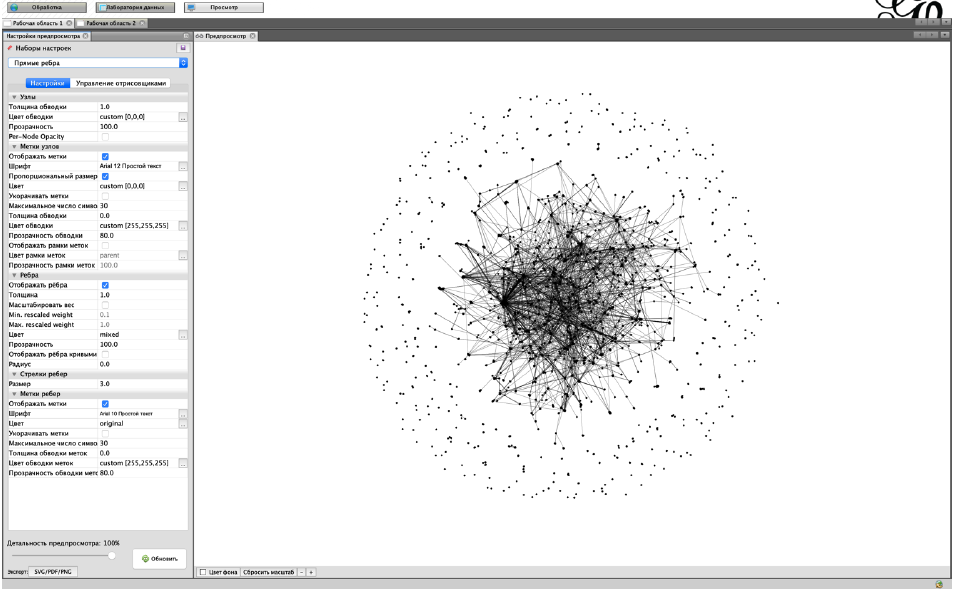
\includegraphics[scale=0.5]{openord.png}
		\caption{OpenOrd layout.}
		\label{openord}
	\end{figure} 
	
	\begin{figure}[h!]
		\centering
		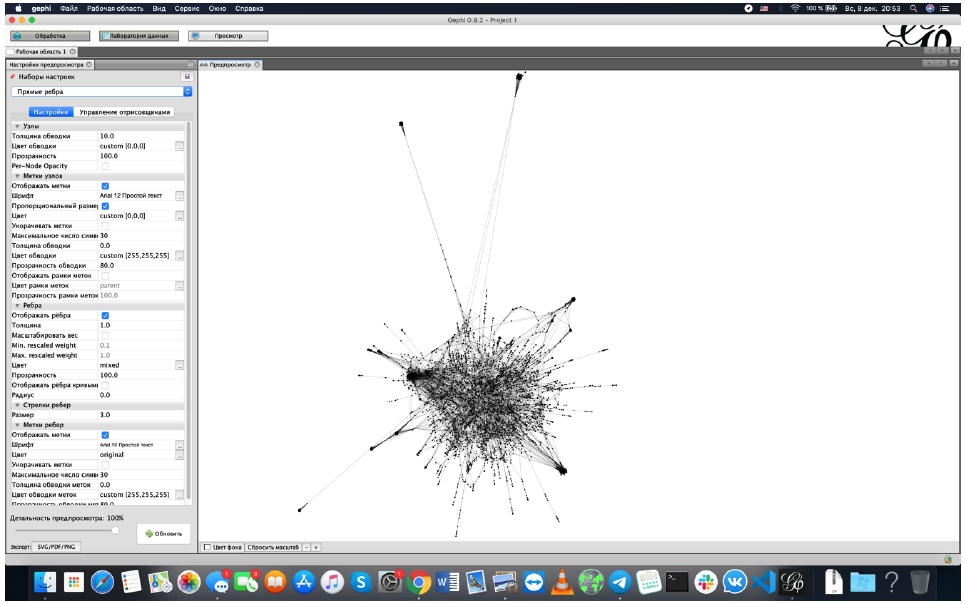
\includegraphics[scale=0.5]{forceatlas.png}
		\caption{ForceAtlas2 layout.}
		\label{force}
	\end{figure}
	
	\begin{figure}[h!]
		\centering
		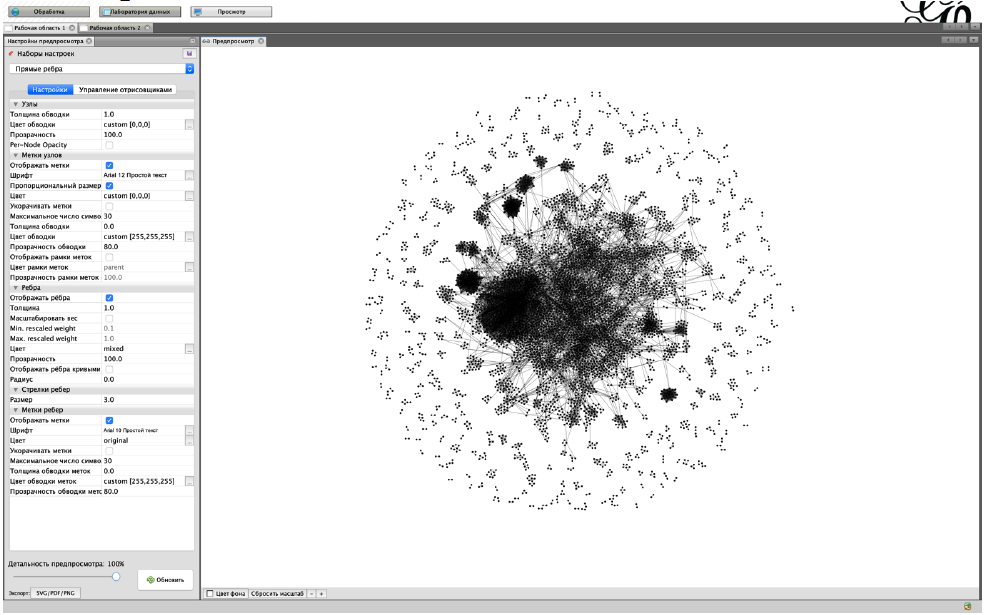
\includegraphics[scale=0.5]{noverlap.png}
		\caption{Noverlap layout.}
		\label{noverlap}
	\end{figure}
	
\end{document}